\documentclass{beamer}

%\usetheme{Madrid}
%\usetheme{Boadilla}
%\usetheme{default}
%\usetheme{Warsaw}
%\usetheme{Bergen}
%\usetheme{Frankfurt}
\usetheme{Darmstadt}

\setbeamercolor{normal text}{fg=white}
\setbeamertemplate{background canvas}[vertical shading] [top=black!95,bottom=black!65]

\definecolor{mypurple}{RGB}{207,78,64}
\usecolortheme[named=mypurple]{structure}

\definecolor{myorange}{RGB}{255,235,190}
\beamerboxesdeclarecolorscheme{orange}{orange}{myorange}

\definecolor{commandcolor}{RGB}{111,195,165}

\setbeamertemplate{footline}[page number]
%\setbeamercovered{transparent}
\setbeamercovered{invisible}
\setbeamertemplate{navigation symbols}{}

%\usepackage{musixtex}
\usepackage{multimedia}
\usepackage{graphicx}
\usepackage[utf8]{inputenc}
%\usepackage[T1]{fontenc}
\usepackage[french]{babel} 
%\usepackage[all]{xy}
%\usepackage{multirow}
%\usepackage{lmodern}
\usepackage{subfigure}
%\usepackage{ulem}
\usepackage{url}
\usepackage{hyperref}
\usepackage{verbatim}
\usepackage{xspace}
\usepackage{color}
\usepackage{xcolor}
\usepackage{rotating}
\usepackage{multicol}
\usepackage[export]{adjustbox}
\usepackage{textpos}
\usepackage{listings}
\usepackage{fontawesome}


\definecolor{mypurple}{RGB}{207,78,64}
\usecolortheme[named=mypurple]{structure}

\definecolor{myorange}{RGB}{255,235,190}
\beamerboxesdeclarecolorscheme{orange}{orange}{myorange}

\definecolor{dgreen}{RGB}{0,125,0}

\usepackage{tikz}
\usetikzlibrary{trees}

\setbeamertemplate{caption}[numbered] 

\newcommand{\setframetitle}[1]{\begin{center}
    \huge \textbf{#1}
\end{center}}


%% --------------

\title{Atelier d'aide à la programmation}
\subtitle{Partage de compétences}
\author{L\'eo \textsc{Baudouin}}
\institute{
  {\url{baudouin.leo @ gmail.com}}
}
\date{19-20 juin 2025}




%% --------------

\begin{document}

\begin{frame}
  \titlepage
\end{frame}



%-------

\section{Gestion de projet}
\subsection{}

\begin{frame}{Gestion de projet informatique}
\begin{center}
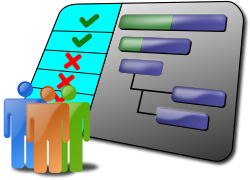
\includegraphics[width=0.5\linewidth]{images/project}

\end{center}
\end{frame}




\begin{frame}
  \frametitle{Partage de codes-sources}
  \textbf{Exemple :} Partage d'une bibliothèque
  
  \begin{figure}
    \begin{tikzpicture}[scale=1.0]
      \tikzset{mypoints/.style={fill=white,draw=black,thick}}
      \def\ptsize{1.0pt}
      
      \tikzset{dev/.style={rectangle,draw,color=cyan}}
      \tikzset{unk/.style={rectangle,draw,color=red,rounded corners=.8ex}}
      \tikzset{lib/.style={rectangle,draw,color=orange,rounded corners=.8ex}}
      \tikzset{proj/.style={rectangle,draw,color=green,rounded corners=.8ex}}
      \tikzset{version/.style={rectangle,draw,color=gray,rounded corners=.8ex}}
      \tikzset{branch/.style={grow=down,xshift=1em,anchor=west,   edge from parent path={(\tikzparentnode.south) |- (\tikzchildnode.west)}}}
      \tikzset{first/.style={level distance=5ex}}
      \tikzset{second/.style={level distance=10ex}}
      \tikzset{grow=right}
      \tikzset{arrow/.style={edge from parent/.style={draw,-latex}}}
      
      \coordinate
      node[dev]{Dev1}
       child[arrow] {node[lib]{lib}
        child { node[proj]{Projet1} }
      child[arrow] { node[unk]{$???$}
        child { node[dev]{Dev2}
  	  child[level distance=13ex] { node[proj]{Projet2} 
            child[grow=south,first,branch] { node[version] {Version 1}}
            child[grow=south,second,branch] { node[version] {Version 2}}
  	  } 
        }
        child { node[dev]{Dev3} 
          child[level distance=12ex] { node[proj]{Projet3} }
        }
      }
      };
    \end{tikzpicture}
  \end{figure}
\end{frame}


\begin{frame}{Partage de codes-sources}
  
  \vspace{5mm}
  \textbf{Exemple :} Partage d'une bibliothèque
  \begin{figure}
    \begin{tikzpicture}[scale=1.0]
      \tikzset{mypoints/.style={fill=white,draw=black,thick}}
      \def\ptsize{1.0pt}
      
      \tikzset{dev/.style={rectangle,draw,color=cyan}}
      \tikzset{lib/.style={rectangle,draw,color=orange,rounded corners=.8ex}}
      \tikzset{proj/.style={rectangle,draw,color=green,rounded corners=.8ex}}
      \tikzset{commit/.style={rectangle,draw,color=gray,rounded corners=.8ex}}
      \tikzset{final/.style={circle,draw,color=orange}}
      
      \node[lib] (lib) {lib};
      \node[proj] (p2) [below of=lib,yshift=-5mm] {Projet2};
      \node[proj] (p3) [below of=p2,yshift=-5mm] {Projet3};
      
      \node[commit] (e1) [right of=lib,xshift=7mm] {$C_{1,1}$};
      \node[commit] (e2) [right of=e1,xshift=5mm] {$C_{1,2}$};
      \node[commit] (e3) [right of=e2,xshift=8mm] {$C_{1,3}$};
      
      \node[commit] (v1) [below of=e2,yshift=-20mm] {$C_{3,1}$};
      \node[commit] (v2) [right of=v1] {$C_{3,2}$};
      \node[commit] (v3) [right of=v2] {$C_{3,3}$};
      
      \node[commit] (s1) [below of=e1,yshift=-5mm,xshift=5mm] {$C_{2,1}$};
      \node[commit] (s2) [below of=e3,yshift=-5mm,xshift=-5mm] {$C_{2,2}$};
      
      \node[final] (end) [right of=e3,xshift=8mm] {}; 
      \node[final] (endv) [below of=end,yshift=-20mm] {}; 
      \node[final] (ends) [below of=end,yshift=-5mm] {}; 
      
      \node[dev] (dlib) [above of=lib] {Dev1};
      \node[dev] (ddj) [left of=p2,xshift=-10mm] {Dev2};
      \node[dev] (ddd) [left of=p3,xshift=-10mm] {Dev3};
      \node[dev] (de) [above of=e1] {Dev1};
      \node[dev] (dj) [above of=e2] {Dev2};
      \node[dev] (dd) [above of=e3] {Dev3};
      
      \draw[->,dashed] (lib) -- (e1);
      \draw[->,dashed] (e1) -- (e2);
      \draw[->,dashed] (e2) -- (e3);
      \draw[->,dashed] (e3) -- (end);
      
      \draw[->,dashed] (p3) -- (v1);
      \draw[->,dashed] (v1) -- (v2);
      \draw[->,dashed] (v2) -- (v3);
      \draw[->,dashed] (v3) -- (endv);
      
      \draw[->] (dlib) -- (lib);
      \draw[->,dashed] (p2) -- (s1);
      \draw[->,dashed] (s1) -- (s2);
      \draw[->,dashed] (s2) -- (ends);
      
      
      \draw[->] (de) -- (e1);
      \draw[->] (dj) -- (e2);
      \draw[->] (dd) -- (e3);
      \draw[->] (ddj) -- (p2);
      \draw[->] (ddd) -- (p3);
      
      \draw[double,red,->] (endv) .. controls ([xshift=+5mm,yshift=-15mm] end) .. (end);
      \draw[double,red,->] (ends) .. controls ([xshift=-3mm,yshift=8mm] ends) .. (end);
      
      \node (legendl) [below of=p3,yshift=-5mm] {};
      \node (legendr) [right of=legendl] {};
      \node (legend) [right of=legendr] {Lié avec};
      
      \draw[red,->]  (legendl) -- (legendr);
      
	  \node (legend_tl) [above of=legendl,left of=legendl,xshift=10mm,yshift=-6mm] {};
	  \node (legend_tr) [right of=legend_tl,xshift=20mm] {};
	  \node (legend_bl) [below of=legend_tl,yshift=2mm] {};
	  \node (legend_br) [right of=legend_bl,xshift=20mm] {};
      
      \draw[dashed] (legend_tl) -- (legend_tr) -- (legend_br) -- (legend_bl) -- (legend_tl);
      
      
    \end{tikzpicture}
  \end{figure}
\end{frame}

\begin{frame}
  \frametitle{Gestion de projet informatique}
  \begin{block}{Besoins}
  \begin{itemize}
  \item Gestion du code source
  \item Wiki
  \item Rapport de bug
  \item Gantt
  \item Historique des modifications/versions
  \item Règles de codage (code style)
  \end{itemize}
  \end{block}
\pause
	\begin{exampleblock}{Solutions}
	\begin{itemize}
	\item Redmine $\Rightarrow$ \url{https://forge.uca.fr/}
	\item Jira, Github, GitLab, \dots
	\item Bitbucket, Trac, Mantis, \dots
	\end{itemize}
	\end{exampleblock}  
  
\end{frame}

\section{Outils}
\subsection{Principaux outils libres}

\begin{frame}
  \frametitle{Les outils}


\begin{block}{Utilisation d'outils de base}


\begin{textblock*}{5cm}(1cm,2cm) 

\includegraphics[max size={32px}{32px}]{images/terminal}
\end{textblock*}

\begin{textblock*}{5cm}(3cm,3cm) 

\includegraphics[max size={32px}{32px}]{images/git-logo}
\end{textblock*}

\begin{textblock*}{5cm}(5cm,2cm) 

\includegraphics[max size={32px}{32px}]{images/cmake}
\end{textblock*}

\begin{textblock*}{5cm}(9cm,2.5cm) 

\includegraphics[max size={45px}{45px}]{images/doxygen}
\end{textblock*}

\begin{textblock*}{5cm}(7.5cm,3cm) 
\LaTeX
\end{textblock*}

\begin{textblock*}{5cm}(1cm,4cm) 

\includegraphics[max size={32px}{32px}]{images/docker}
\end{textblock*}

\begin{textblock*}{5cm}(9cm,4cm) 

\includegraphics[max size={32px}{32px}]{images/qt}
\end{textblock*}

\begin{textblock*}{5cm}(4cm,1cm) 

\includegraphics[max size={32px}{32px}]{images/gdb.jpg}
\end{textblock*}

\begin{textblock*}{5cm}(7cm,1cm) 

\includegraphics[max size={32px}{32px}]{images/qtcreator}
\end{textblock*}

\begin{textblock*}{5cm}(9.5cm,0.5cm) 

\includegraphics[max size={32px}{32px}]{images/kdevelop}
\end{textblock*}

\begin{textblock*}{5cm}(6cm,4cm) 
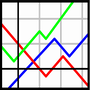
\includegraphics[max size={32px}{32px}]{images/gnuplot}
\end{textblock*}

\begin{textblock*}{5cm}(0.5cm,0.5cm) 

\includegraphics[max size={32px}{32px}]{images/gitlab}
\end{textblock*}

\raisebox{0px}[5.5cm][0cm]{}

\end{block}
  
\end{frame}




\section{Git}
\subsection{Gestion de versions}

\begin{frame}
  \frametitle{Git}

    \begin{figure}
    
\includegraphics[height=0.7\textheight]{images/branches}
    \end{figure}

\end{frame}


%-------

\section{CMake}
\subsection*{Compilation de programmes}

\begin{frame}[label=cmake]
  \frametitle{CMake}
  
    \begin{block}{Aide à la compilation}
    \begin{columns}
      \begin{column}{0.2\linewidth}
        
\includegraphics[width=1\linewidth]{images/compiler.png}
      \end{column}
      \hspace{-15mm}
      \begin{column}{0.7\linewidth}
        \begin{itemize}
        \item Projet multi-plateformes :\linebreak
        Linux / Mac / Windows
        \item Recherche automatique des dépendances
        \item Configuration des projets
        \item Pas de \textbf{makefile} à la main
        \end{itemize}
      \end{column}
      \end{columns}
	\end{block}

    \begin{exampleblock}{Bonus}
    Projet vierge prêt à la compilation et au déploiement
    \end{exampleblock}
\end{frame}

%-------



%-------
\section{Doxygen}
\subsection*{Documentation automatique}

\begin{frame}[fragile,label=doxygen]
  \frametitle{Doxygen}
  \vbox to 0.8 \textheight{
   \begin{exampleblock}{Utilisation}
    Documentation automatique / création d'un site web
   \end{exampleblock}



    \begin{block}{Exemple C++ :}
    \begin{tiny}
  \begin{lstlisting}[language=C++]
  /**
  Apply a rotation to a transformation.
  \f[ m \leftarrow m \times \exp \left(\begin{array}{ccc}
      0 & -z & y \\ z & 0 & -x \\ -y & x & 0 \end{array}\right) \f]
  */
  
  LIBV_GEOMETRY_EXPORT void apply_rotation
  ( Matrix3d &m ///< A transformation matrix.  
  , const Vector3d &d ///< A rotation in axis-angle representation.
    )
  {
    Matrix3d skrew;
    skrew << 0, -d.z(), d.y(), d.z(), 0, -d.x(), -d.y(), d.x(), 0;
    m *= skrew.exp();
  }
\end{lstlisting}
      \end{tiny}
    \end{block}

    \vfill

  }
\end{frame}

\begin{frame}
  \frametitle{Doxygen}
    \begin{block}{Rendu :}
    \begin{figure}
      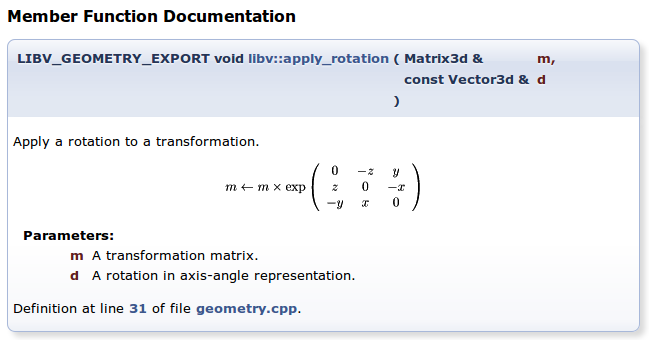
\includegraphics[width=0.9\linewidth]{images/doxygen_sample}  
    \end{figure}
    \end{block}

\end{frame}

%-------------------------------------------------------------------
\end{document} 
%-------------------------------------------------------------------

%\transdissolve[duration=0.25]
%
%\begin{exampleblock}{Avantages}
%\end{exampleblock}
%
%\begin{alertblock}{Inconvénients}
%\end{alertblock}
